% -*- coding: utf-8 -*-
\documentclass{article}

\usepackage{listings}
\usepackage{ctex}
\usepackage{graphicx}
\usepackage[a4paper, body={18cm,22cm}]{geometry}
\usepackage{amsmath,amssymb,amstext,wasysym,enumerate,graphicx}
\usepackage{float,abstract,booktabs,indentfirst,amsmath}
\usepackage{array}
\usepackage{booktabs} %调整表格线与上下内容的间隔
\usepackage{multirow}
\usepackage{diagbox}
\usepackage[colorlinks,linkcolor=blue,urlcolor=black,anchorcolor=blue,citecolor=blue,]{hyperref}%超链接包
\renewcommand\arraystretch{1.4}
\usepackage{indentfirst}
\setlength{\parindent}{2em}

\geometry{left=2.8cm,right=2.2cm,top=2.5cm,bottom=2.5cm}
%\geometry{left=3.18cm,right=3.18cm,top=2.54cm,bottom=2.54cm}

\graphicspath{{figures/}}

\title{\heiti 实验三:GO富集分析}

\begin{document}

	\maketitle
	
	\vspace{5cm}
	
	\begin{table}[h]
		\centering
		\begin{Large}
			\begin{tabular}{p{3cm} p{7cm}<{\centering}}
				学  \qquad  校: &  华中农业大学     \\ \cline{2-2}
				学院班级:      & 信息学院生信1801班   \\ \cline{2-2}
				姓  \qquad  名: & 邓启东 \\ \cline{2-2}
				学  \qquad  号: & 2018317220103 \\ \cline{2-2}
				指导教师:       &夏静波 \\ \cline{2-2}
			\end{tabular}
		\end{Large}		
	\end{table}
	
	\newpage%一个新的页面

	\tableofcontents
	
	\newpage
\section{实验目的}
使用clusterProfiler包进行GO、KEGG的富集分析方法,结果输出及内置的图形展示。
\section{实验材料与方法}
\subsection{GO(Gene Ontology)介绍}
GO是Gene Ontology的简称,是基因功能国际标准分类体系。它旨在建立一个适用于各种物种的,对基因和蛋白质功能进行限定和描述的,并能随着研究不断深入而更新的语言词汇标准。GO分为分子功能(Molecular Function)、生物过程(Biological Process)、和细胞组成(Cellular Component)三个部分。
\subsubsection{基因注释数据库KEGG}
京都基因与基因组百科全书 (Kyoto encyclopedia of genes and genomes, KEGG),是系统分析基因功能与基因组信息的数据库,它整合了基因组学、生物化学和系统功能组学的信息,有助于研究者把基因及表达信息的过程作为一个网络进行整体研究。
\subsection{获取差异表达基因数据}
\subsubsection{阿兹海默症(AD)简介}
阿尔茨海默症(Alzheimer's disease, AD),俗称“老年痴呆症”,是当今世界范围内患病最广泛、病情最严重的神经退行性疾病,患者通常会出现以记忆力衰退、学习能力减弱为主的症状,并伴有情绪调节障碍以及运动能力丧失,极大地影响个人、家庭乃至社会的发展。
\subsubsection{差异基因数据来源}
我们的差异基因来自埃默里大学医学院发表的一篇文章,团队运用全蛋白质组关联研究(proteome-wide association study,PWAS),将阿尔茨海默症(AD)队列 GWAS结果与人脑蛋白质组进行了整合,旨在鉴定通过影响脑蛋白丰度而导致AD风险的基因,深入了解这些基因座如何影响AD的发病机制\cite{2020Integrating}。\par
该研究团队鉴定了11个与AD发病相关的基因,它们通过顺式调节的脑蛋白丰度发挥作用。9个在PWAS验证队列中重现。我们的差异基因正是这已知的九种。\par
根据map的结果显示 有22.22\% 的基因没有得到相应的ENTREZID,分别是"CARHSP","STX"这两个基因。最终的差异表达基数据输入为7个。
\subsection{背景基因获取}
如果clusterProfiler包没有所需要物种的内置数据库,可以通过自定义注释文件或者自建注释库的方法进行富集分析。待富集的背景基因是由函数:list data(geneList, package)获取的,这里使用的是"DOSE"这个库。
\subsection{富集原理}
根据挑选出的差异基因,计算这些差异基因同GO分类中某(几)个特定的分支的超几何分布关系,GO 分析会对每个有差异基因存在的GO Term返回一个假定值p-value,小的p 值表示差异基因在该GO 中出现了富集。
\section{结果及分析}
\subsection{差异表达基因GO富集分析}
GO富集分析结果主要由有向无环图DAG和柱状图两种形式所表示。
\subsubsection{DAG}
得到的有向无环图如下图\ref{xxxxxx}所示。结果中箭头"$\rightarrow$"代表GO\quad term的上下层级关系,圆圈代表富集程度未在前十的GO\quad term,方格代表富集程度在前十的GO\quad term。\par
图形的颜色反应了基因在某一个GO Term上的富集程度,颜色越深代表富集程度越显著。GO Term的层级越低,功能描述越具体。
\begin{figure}[H]
  \centering
  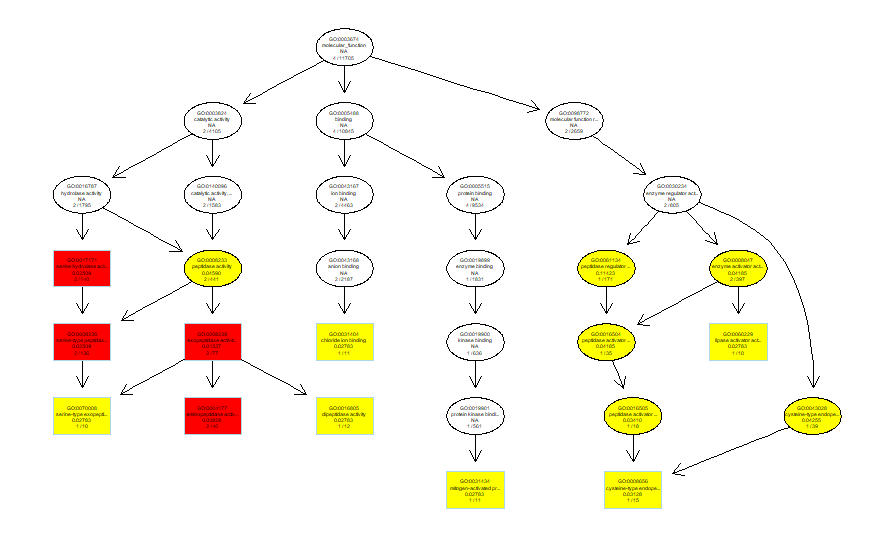
\includegraphics[scale=0.5]{./picture/Rplot.png} %1.png是图片文件的相对路径
  \caption{差异表达基因富集分析DAG图} %caption是图片的标题
  \label{xxxxxxx} %此处的label相当于一个图片的专属标志,目的是方便上下文的引用
\end{figure}
\subsubsection{柱状图}
柱状图结果如下图(图\ref{xxxasddf})所示:
\begin{figure}[H]
  \centering
  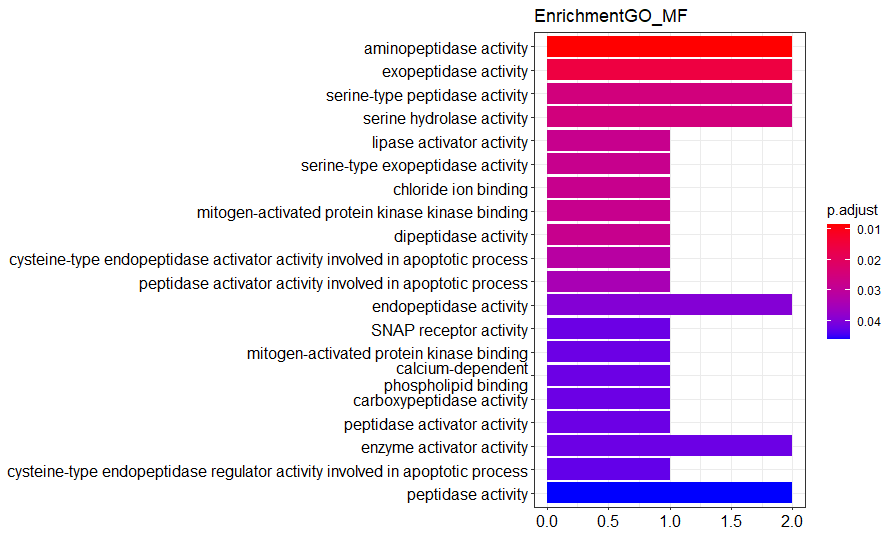
\includegraphics[scale=0.48]{./picture/Rplot01.png} %1.png是图片文件的相对路径
  \caption{差异表达基因富集分析柱状图} %caption是图片的标题
  \label{xxxasddf} %此处的label相当于一个图片的专属标志,目的是方便上下文的引用
\end{figure}
可以看到富集结果按照按照p值排名前十的分别是:\par
aminopeptidase activity(氨肽酶活性)、exopeptidase activity(外肽酶的活动)、serine type peptidase activity(丝氨酸型肽酶活性)、lipase activator activity(脂肪酶催化剂活性)、serine type exopeptidase activity(丝氨酸型外肽酶活性)、chloride ion binding(氯离子结合)、mitogen activated protein kinase kinase binding(丝裂原激活蛋白激酶激酶结合)、dipeptidase activity(二肽酶的活动)、cysteine-type endopeptidase activator activity involved in apoptotic process(半胱氨酸型内肽酶激活物活性参与凋亡过程)、endopeptidase activity(肽链内切酶活性)。\par
可以观察发现这个当中基本上每一个都涉及到酶的活性。通过相关文献检索发现,事实上阿兹海默症的确和酶的活性、结合有关。例如施一公团队发现了阿尔兹海默重要蛋白γ分泌酶\cite{2020Structural}。该酶便能水解淀粉样蛋白。而阿兹海默症的症状之一就是淀粉样沉积。\par
关于出现的第六条氯离子结合,我们也在一个电分析化学学术会议文章中找到证据,通过微传感用于AD及缺血模型下鼠脑中三个脑区(海马,纹状体,皮层)Cl~–的测定,发现氯离子(Cl~–)作为人体常见的阴离子在AD的病理过程起着重要作用\href{http://cpfd.cnki.com.cn/Article/CPFDTOTAL-ZGHY201704002184.htm}{\underline{(链接)}}\par
其中的肽链内切酶活性,也可以找到相应证据:天冬酰胺内肽酶(asparagine endopeptidase,AEP)也被称为豆荚蛋白,它是一个溶酶体半胱氨酸蛋白酶,能够将蛋白c端的天冬氨酸剪切掉。编码AEP基因缺失的tau P301s转基因小鼠,其tau的过度磷酸化被降低,突触损害降低以及认知障碍得到改善。这些结果表明,AEP在AD中发挥了关键作用,抑制AEP或许能 够成为治疗AD的有效方法\cite{2021Pharmacological}。
\section{结论与展望}
本次实验,从文献当中找到了GWAS、PWAS等方法通过测序得到的一些阿兹海默的关联基因,但是由于GWAS的假阳性等以及缺乏证据等原因,这些基因还有待于进一步证实。通过基因富集分析,我们能够了解到这些突变位点具体和哪些分子层面的性状有关,这些性状再经过人工的文献检索,发现的确已经有相关工作作为证据表明其确实与疾病相关联。也印证了这一套基因富集分析的流程有利于我们发现疾病的一些潜在机理。\par
当然我们现在是拿着结果在验证。如果发现了新的知识,光靠富集分析还不足以作为可信的证据,有待后续进一步的分析和确认。
\section{Github链接}
\href{https://github.com/LianzePuppet/nlphomework3}{\underline{github链接:}}https://github.com/LianzePuppet/nlphomework3
\bibliographystyle{unsrt}
\bibliography{MyCitation}% Produces the bibliography via BibTeX.
\end{document}



















%%%%%%%%%%%%%%%%%%%%%%%%%%%%Library%%%%%%%%%%%%%%%%%%%%%%%%%%%%%%%%%%%%%%%

% 1. 脚注用法
	LaTeX\footnote{Latex is Latex} is a good software

%2. 强调
	\emph{center of percussion} %[Brody 1986], %\lipsum[5]

%3. 随便生成一段话
	\lipsum[4]

%4. 列条目
	\begin{itemize}
	\item the angular velocity of the bat,
	\item the velocity of the ball, and
	\item the position of impact along the bat.
	\end{itemize}

%5. 表格用法
	\begin{table}[h]
	\centering  
	\begin{tabular}{c|cc}
		\hline
		年份 & \multicolumn{2}{c}{指标}\\
		\hline
		2017 & 0.9997 & 0.0555 \\
		2018 & 0.9994 & 0      \\
		2019 & 0.9993 & 0      \\
		\hline
	\end{tabular}
	\caption{NAME}\label{SIGN}
	\end{table}

	\begin{center}
		\begin{tabular}{c|cclcrcc}
			\hline
			Year & theta & $S_1^-$ & $S_2^-$ & $S_3^-$ & $S_4^+$ & $S_5^+$ & $S_6^+$ \\%表格标题
			\hline
			2016 & 1      & 0      & 0 & 0.0001 & 0      & 0      & 0 \\
			2017 & 0.9997 & 0.0555 & 0 & 0.2889 & 0.1844 & 0.463  & 0 \\
			2018 & 0.9994 & 0      & 0 & 0.0012 & 0.3269 & 0.7154 & 0 \\
			2019 & 0.9993 & 0      & 0 & 0      & 0.4325 & 1.0473 & 0 \\
			2020 & 0.9991 & 0      & 0 & 0      & 0.5046 & 1.2022 & 0 \\
			2021 & 0.999  & 0      & 0 & 0      & 0.5466 & 1.2827 & 0 \\
			2022 & 0.9989 & 0.0017 & 0 & 0.3159 & 0.562  & 1.2995 & 0 \\
			2023 & 0.9989 & 0      & 0 & 0.0109 & 0.5533 & 1.2616 & 0 \\
			2024 & 0.9989 & 0      & 0 & 0      & 0.5232 & 1.1769 & 0 \\
			2025 & 0.9989 & 0      & 0 & 0.1009 & 0.4738 & 1.0521 & 0 \\
			2026 & 0.9991 & 0      & 0 & 0      & 0.4071 & 0.8929 & 0 \\
			2027 & 0.9992 & 0.0004 & 0 & 0.1195 & 0.3248 & 0.7042 & 0 \\
			2028 & 0.9994 & 0.0164 & 0 & 0.046  & 0.2287 & 0.4902 & 0 \\
			2029 & 0.9997 & 0      & 0 & 0.0609 & 0.12   & 0.2545 & 0 \\
			2030 & 1      & 0      & 0 & 0      & 0      & 0      & 0 \\
			\hline
		\end{tabular}
	\end{center}

%6. 数学公式
	\begin{equation}
		a^2 = a * a\label{aa}
	\end{equation}
	
	\[
	\begin{pmatrix}{*{20}c}
	{a_{11} } & {a_{12} } & {a_{13} }  \\
	{a_{21} } & {a_{22} } & {a_{23} }  \\
	{a_{31} } & {a_{32} } & {a_{33} }  \\
	\end{pmatrix}
	= \frac{{Opposite}}{{Hypotenuse}}\cos ^{ - 1} \theta \arcsin \theta
	\]
	
	\[
	p_{j}=\begin{cases} 0,&\text{if $j$ is odd}\\
	r!\,(-1)^{j/2},&\text{if $j$ is even}
	\end{cases}
	\]
	
	
	\[
	\arcsin \theta  =
	\mathop{{\int\!\!\!\!\!\int\!\!\!\!\!\int}\mkern-31.2mu
		\bigodot}\limits_\varphi
	{\mathop {\lim }\limits_{x \to \infty } \frac{{n!}}{{r!\left( {n - r}
				\right)!}}} \eqno (1)
	\]

%7. 双图并行
	\begin{figure}[h]
		% 一个2*2图片的排列
		\begin{minipage}[h]{0.5\linewidth}
			\centering
			\includegraphics[width=0.8\textwidth]{./figures/0.jpg}
			\caption{Figure example 2}
		\end{minipage}
		\begin{minipage}[h]{0.5\linewidth}
			\centering
			\includegraphics[width=0.8\textwidth]{./figures/0.jpg}
			\caption{Figure example 3}
		\end{minipage}
	\end{figure}

%8. 单张图片部分
	\begin{figure}[h]
		%\small
		\centering
		\includegraphics[width=12cm]{./figures/mcmthesis-aaa.eps}
		\caption{Figure example 1} \label{fig:aa}
	\end{figure}

%%%%%%%%%%%%%%%%%%%%%%%%%%%%%%%%%%%%%%%%%%%%%%%%%%%%%%%%%%%%%%%%%%%%%%%%%%%%%
\begin{minipage}{0.5\linewidth}
	\begin{tabular}{|c|c|c|}
		\hline
		\multicolumn{2}{|c|}{\multirow{2}{*}{合并}}&测试\\
		\cline{3-3}
		\multicolumn{2}{|c|}{}& 0.9997  \\
		\hline
		2019 & 0.9993 & 0 \\
		\hline
	\end{tabular}
\end{minipage}

\begin{minipage}{0.5\linewidth}
	\begin{tabular}{c|ccc}
		\hline
		年份 & \multicolumn{3}{c}{指标}\\
		\hline
		\multirow{3}{*}{合并}&2017 & 0.9997 & 0.0555 \\
		&2018 & 0.9994 & 0      \\
		&2019 & 0.9993 & 0      \\
		\hline
	\end{tabular}
\end{minipage}



	\begin{table}[h]
	\centering	
	\begin{Large}
		\begin{tabular}{p{4cm} p{8cm} < {\centering}}
			\hline
			院\qquad 系: & 信息工程学院 \\
			\hline
			团队名称: & PlantBook Team \\
			\hline
			分\qquad 组: & 第0组1号 \\
			\hline
			日\qquad 期: & 2017年10月28日 \\
			\hline
			指导教师: & 吱吱吱\\
			\hline
		\end{tabular}
	\end{Large}
\end{table}


\ctexset{
	section={
		format+=\heiti \raggedright,
		name={,、},
		number=\chinese{section},
		beforeskip=1.0ex plus 0.2ex minus .2ex,
		afterskip=1.0ex plus 0.2ex minus .2ex,
		aftername=\hspace{0pt}
	},
}

	\begin{table}[h]
	\centering
	\begin{Large}
		\begin{tabular}{p{3cm} p{7cm}<{\centering}}
			院  \qquad  系: & 信息工程学院           \\ \cline{2-2}
		\end{tabular}
	\end{Large}		
\end{table}
\thispagestyle{empty}
\newpage
\thispagestyle{empty}
\tableofcontents
\thispagestyle{empty}
\newpage
\setcounter{page}{1}

% 9. 代码

\usepackage{listings}
\usepackage{xcolor}
\lstset{
	numbers=left, 
	numberstyle= \tiny, 
	keywordstyle= \color{ blue!70},
	commentstyle= \color{red!50!green!50!blue!50}, 
	frame=shadowbox, % 阴影效果
	rulesepcolor= \color{ red!20!green!20!blue!20} ,
	escapeinside=``, % 英文分号中可写入中文
	xleftmargin=2em,xrightmargin=2em, aboveskip=1em,
	basicstyle=\footnotesize,
	framexleftmargin=2em
}
